\documentclass[a4paper,chapterprefix]{scrbook}
\usepackage[english]{babel}
\usepackage{fullpage}
\usepackage{tabularx,booktabs}
\usepackage{graphicx}
\usepackage{import}
\usepackage{hyperref}
\usepackage{listings}
\usepackage{xcolor}
\usepackage{multirow}
%\usepackage{titlesec}
%\titleformat{\section}
%  {\normalfont\Large\bfseries}{\thesection}{1em}{}[{\titlerule[0.8pt]}]


\colorlet{chaptercolor}{blue!80!black}

\setkomafont{chapter}{\normalfont\Huge\color{gray}\bfseries}
\setkomafont{chapterprefix}{\Large}
\renewcommand*{\raggedchapter}{\raggedleft}
\renewcommand*{\chapterformat}{%
  \MakeUppercase{\chapappifchapterprefix{}}%
  \enskip\resizebox{!}{2cm}{\thechapter} \rlap{\rule{10cm}{1.2cm} }%
}

\RedeclareSectionCommand[beforeskip=30pt,afterskip=50pt]{chapter}
\renewcommand*\chapterheadmidvskip{\par\nobreak\vspace{10pt}}


\definecolor{codegreen}{rgb}{0,0.6,0}
\definecolor{codegray}{rgb}{0.5,0.5,0.5}
\definecolor{codepurple}{rgb}{0.58,0,0.82}
\definecolor{backcolour}{rgb}{0.95,0.95,0.95}
 
\lstdefinestyle{myObjCstyle}
{
    language=[Objective]C,
    basicstyle=\ttfamily\small,
    keywordstyle=\color{blue},
    backgroundcolor=\color{backcolour},   
    commentstyle=\color{codegreen},
    %keywordstyle=\color{magenta},
    numberstyle=\tiny\color{codegray},
    stringstyle=\color{codepurple},
    basicstyle=\footnotesize,
    breakatwhitespace=false,         
    breaklines=true,                 
    captionpos=b,                    
    keepspaces=true,                 
    numbers=left,                    
    numbersep=5pt,                  
    showspaces=false,                
    showstringspaces=false,
    showtabs=false,                  
    tabsize=2,
    morekeywords={
    		ARM_MAIN_FUNCTION,
    		SPHERE,
    		LAMBERT_EMITTER,
    		CAMERA,
    		IVEC2D,
    		RAY3D,
    		PNT3D, PNT3D_HUGE,
    		VEC3D,
    		ACTION_SEQUENCE,
    		CREATE_STANDARD_RAYCASTING_ACCELERATION_STRUCTURE,
    		STOCHASTIC_PIXEL_SAMPLER,
    		SIMPLE_PATHTRACER,
		PATHTRACER,
    		STANDARD_RAYCASTER,
    		TENT_KERNEL,
    		RANDOM_SEQUENCE,
    		ACTION_SEQUENCE_END,
    		IMAGECONVERSION_ARTRAW_TO_ARTCSP,
    		STANDARD_TONEMAPPING_OPERATOR,
		STANDARD_GLOBAL_TONEMAPPING_OPERATOR,
		STANDARD_LUMINANCE_CLIPPING,
    		IMAGECONVERSION_ARTCSP_TO_TIFF,
    		YES, NO,
    		SCENE,
		DEGREES, NANOMETER,
		LIGHTSOURCE_COLLECTOR,
		STANDARD_SAMPLER_2D,
		ArObj, ART_GV, Pnt3D,
		ALLOC_ARRAY,
		CONST_COLOUR_RSSPECTRUM,
		RSS_END,
		LAMBERT_REFLECTOR_CONST,
		QUADRANGLE, 
		UNION,
		UNION_END,
		UNIFORM_ENVIRONMENT_MATERIAL,
		CONST_COLOUR_GREY,
		}
}
\lstset{style=myObjCstyle, breakindent=40pt, breaklines}

\title{
  \Huge ART - The Advanced Rendering Toolkit
  %\newline
  %\newline
  %\Large ARM Scene File Interface
}
\subtitle{ARM Scene File Interface}
\date{}

\begin{document}
\maketitle
\tableofcontents

\part{Writing an ART scene}

\chapter{Your first ART scene}

ART uses the \verb?.arm? file format to describe scenes. These files contain Objective-C code which is compiled and linked against the ART library: the exact process is described in section~8.3 of the ART Handbook. To write ARM files, a set of convenience functions and defines are available which allow easy access to the various scene graph elements defined in ART. To process such scenes, one then simply use the \verb?artist? executable, which will compile and render the results of the ARM file. The purpose of this document is to provide an overview of the pre-defined constructor functions which one can use in ARM files.

\section{Basic structure of an ARM file}
Every ARM file must provide a main function, which is declared like so:
\begin{lstlisting}
ARM_MAIN_FUNCTION(SceneName)
{
    ...
}
\end{lstlisting}

This function must return an instance of \verb?ArnScene?, which is an Objective-C class that defines the root object of ART scenegraphs. To define such an object, one uses the macro \verb?SCENE?, plus the following parameters:

\begin{itemize}
	\item The geometry of the scene: this includes definitions of scene appearance (surface and volume materials)
	\item A camera object
	\item An \emph{action sequence}, which is a list of processing steps that ART will execute to process the scene
\end{itemize}

\begin{lstlisting}
ARM_MAIN_FUNCTION(SceneName)
{
    ...
    return 
        [ SCENE
            sceneGeometry:  scene_geometry
            camera:         camera
            actionSequence: actionsquence
            ];
}
\end{lstlisting}

\section{Scene geometry}
Now, let's create simple scene consisting in a sphere emitting light. To create a sphere, you can use the define \verb?SPHERE?. This will create an Objective-C object. 

You can then assign to this sphere various properties using the method \verb?apply?.
In our case, we are going to assign to our geometry a surface material: a Lambert emitter that can be created using the define \verb?LAMBERT_EMITTER?.

The  \verb?LAMBERT_EMITTER? needs a spectrum of emission, we are going to use a predefined spectrum which is flat over all the wavelengths, \verb?ARNGREY_100?. It also requires a brightness parameter, for this example, we are using 1.0.

\begin{lstlisting}
id scene_geometry = 
    [ SPHERE 
        apply: LAMBERT_EMITTER(ARNGREY_100, 1.0) 
        ];
\end{lstlisting}

\section{Camera}
After having a geometry in our scene, we need a camera to tell the renderer how the scene should be framed. The define \verb?CAMERA? gives us an Objective-C object that then needs to be configured to setup the camera. 

\begin{lstlisting}
id camera =
    [ CAMERA
        imageSize: IVEC2D(250, 250)
        ray:       RAY3D( PNT3D(0.0, 0.0, -5.0), VEC3D(0.0, 0.0, 1.0) )
        zoom:      1
        ];
\end{lstlisting}

\section{Action sequence}
The action sequence can be considered as the brain directing how ART should handle the scene. It specifies a series of actions that need to be performed, which technique should be used to render the scene and what post processing should be done after rendering the scene.

First, let's create a simple action sequence consisting in telling ART to build the ray-casting acceleration structure and then to render the scene using a stochastic pixel sampler which consist in a path tracer.

The ray-casting acceleration structure can be created with the define:\\ \verb?CREATE_STANDARD_RAYCASTING_ACCELERATION_STRUCTURE?.
The stochastic pixel sampler is created with \verb?STOCHASTIC_PIXEL_SAMPLER?. Then, it needs to be initialised with 

\begin{itemize}
	\item a sample provider, in our case a path tracer with direction sampling that we are creating with \verb?SIMPLE_PATHTRACER?. This object needs as well to be parametrised with:
	\begin{itemize}
		\item a raycaster, we are using the \verb?STANDARD_RAYCASTER?
		\item the length of the path, in our case, 8
	\end{itemize}
	\item a kernel for splatting pixels, we are using a \verb?TENT_KERNEL?
	\item the number of samples per pixels, in our case 8
	\item a random value generator, we are using \verb?RANDOM_SEQUENCE? predefined object.
\end{itemize}

\begin{lstlisting}
id actionsquence = 
    ACTION_SEQUENCE(
        CREATE_STANDARD_RAYCASTING_ACCELERATION_STRUCTURE,

        [ STOCHASTIC_PIXEL_SAMPLER
            sampleProvider:
                [ SIMPLE_PATHTRACER
                    rayCaster:        STANDARD_RAYCASTER
                    maximalRecursion: 8
                ]
            sampleSplattingKernel: TENT_KERNEL
            samplesPerPixel:       8
            randomValueGeneration: RANDOM_SEQUENCE
            ],

        ACTION_SEQUENCE_END
        );
\end{lstlisting}

Now, everything is ready to create our very first scene:

\begin{lstlisting}
ARM_MAIN_FUNCTION(SimpleScene)
{
    id scene_geometry = 
        [ SPHERE 
            apply: LAMBERT_EMITTER(ARNGREY_100, 1.0) 
            ];
    id camera =
        [ CAMERA
            imageSize: IVEC2D(250, 250)
            ray:       RAY3D(PNT3D(0.0, 0.0, -5.0), VEC3D(0.0, 0.0, 1.0))
            zoom:      1
            ];
    
    id actionsquence = 
        ACTION_SEQUENCE(
            CREATE_STANDARD_RAYCASTING_ACCELERATION_STRUCTURE,
    
            [ STOCHASTIC_PIXEL_SAMPLER
                sampleProvider:
                    [ SIMPLE_PATHTRACER
                        rayCaster:        STANDARD_RAYCASTER
                        maximalRecursion: 8
                    ]
                sampleSplattingKernel: TENT_KERNEL
                samplesPerPixel:       8
                randomValueGeneration: RANDOM_SEQUENCE
                ],

            ACTION_SEQUENCE_END
            );
    
    return 
        [ SCENE
            sceneGeometry:  scene_geometry
            camera:         camera
            actionSequence: actionsquence
            ];
}
\end{lstlisting}

However, if we render this scene using:

\begin{verbatim}
artist SimpleScene.arm
\end{verbatim}

The renderer will not produce any common image file format. As matter of fact, the renderer will produce an ARTRAW which is the raw output of the renderer. To view it, it needs to be converted to RGB colourspace and tone-mapped. You can do that using \verb?tonemap? utility:

\begin{verbatim}
tonemap SimpleScene.artraw -iac
\end{verbatim}

However, for more convenience, you may want to have the tone-mapped version generated on the fly. This can be done by adding some instructions in the action sequence.

To convert the spectral ARTRAW file to a RGB version, ART is using an intermediate format, ARTCSP. To perform this action, use the object given by \verb?IMAGECONVERSION_ARTRAW_TO_ARTCSP? and tell if you want to retain the ARTRAW file after the conversion. In our case, we want to keep the original file:

\begin{lstlisting}
[ IMAGECONVERSION_ARTRAW_TO_ARTCSP
    removeSource: NO
    ]
\end{lstlisting}

Then, you may want to have the RGB image tone-mapped. For this specific case, it is not necessary but, we can still add this action, with \verb?STANDARD_GLOBAL_TONEMAPPING_OPERATOR?. 
\\

Finally, we want an 8 bit per pixels TIFF image. This time, we don't want to retain the ARTCSP file, so, we are configuring the object to erase this file after the TIFF conversion.

So, we can add the relevant action to perform this task:
\begin{lstlisting}
[ IMAGECONVERSION_ARTCSP_TO_TIFF
    removeSource:    YES
    bitsPerChannel:  8
    ]
\end{lstlisting}

Now, the scene with the updated action sequence should be like so:

\lstinputlisting{Example_Scene/SimpleScene.arm}

Now, if we invoke artist on this file:
\begin{verbatim}
artist SimpleScene.arm
\end{verbatim}

We should obtain at the end of the rendering a file \verb?SimpleScene.tiff?.

\begin{figure}[h]
	\centering
	
\includegraphics[width=0.2\linewidth]{Example_Scene/SimpleScene.png}
	\caption{Rendering result of SimpleScene.arm}
\end{figure}

%%%%%%%%%%%%%%%%%%%%%%%%%%%%%%%%%%%%%%%%%%%%%%%%%%%%%%%%%%%%%%

\chapter{A Cornell Box}
To introduce you to the ARM scene description, let's build a Cornell box from scratch. The specification for the Cornell Box is available here: \url{http://www.graphics.cornell.edu/online/box/data.html}.

So, let's create a new file \verb?CornellBox.arm?.

\section{Camera}
First, we need to create a camera. The Cornell box specifications describes the camera as being position at $(278, 273, -800)$, with the forward direction $(0, 0, 1)$ and the up direction being $(0, 1, 0)$.

However, if we create a camera in ART with those commands:

\begin{lstlisting}
id camera =
    [ CAMERA
        imageSize: IVEC2D(250, 250)
        ray:       RAY3D(PNT3D(278, 273, -800), VEC3D(0.0, 0.0, 1.0))
        zoom:      1
        ];
\end{lstlisting}

We are going to obtain a camera with $(1, 0, 0)$ as the up vector.
So, we just need to modify it doing:

\begin{lstlisting}
[ camera withTwist: -90 DEGREES ];
\end{lstlisting}

\section{Action sequence}
Our action sequence is going to slightly differ from the one used previously:

\begin{itemize}
	\item We are adding a \verb?LIGHTSOURCE_COLLECTOR? since we want to use multiple importance sampling mode for the pathtracer.
	\item We are using a tonemapping operator
	\item We are performing luminance clipping
\end{itemize}

So, our action sequence will be defined like so:
\begin{lstlisting}
id actionsquence = 
    ACTION_SEQUENCE(
        CREATE_STANDARD_RAYCASTING_ACCELERATION_STRUCTURE,
            
        [ LIGHTSOURCE_COLLECTOR
            sampler2D:   STANDARD_SAMPLER_2D
            resolution:  5
            type:        arlightsourcetype_area
            ],

        [ STOCHASTIC_PIXEL_SAMPLER
            sampleProvider:
                [ PATHTRACER
                    rayCaster:        STANDARD_RAYCASTER
                    maximalRecursion: 8
                    mode:             arpathtracermode_mis
                    ]
            sampleSplattingKernel: TENT_KERNEL
            samplesPerPixel:       8
            randomValueGeneration: RANDOM_SEQUENCE
            ],

        [ IMAGECONVERSION_ARTRAW_TO_ARTCSP
            removeSource: NO
            ],

        STANDARD_GLOBAL_TONEMAPPING_OPERATOR,
                        
        STANDARD_LUMINANCE_CLIPPING,
            
        [ IMAGECONVERSION_ARTCSP_TO_TIFF
            removeSource:   YES
            bitsPerChannel: 8
            ],
            
        ACTION_SEQUENCE_END
        );
\end{lstlisting}

\section{Geometry}
Now that we have a camera and an action sequence, we are missing the geometry to have a first scene to render. The materials can be supplied later. To make the work easier, we are going to add temporary an environment lighting. This will help to debug potential error on geometry placement while building the scene.

This can be done by supplying to the scene an \verb?environmentMaterial?:

\begin{lstlisting}
ARM_MAIN_FUNCTION(CornellBox)
{
    ...
    
    return
        [ SCENE
            sceneGeometry:  scene_geometry
            environmentMaterial: UNIFORM_ENVIRONMENT_MATERIAL( CONST_COLOUR_GREY(1.0), 1.0 )
            camera:         camera
            actionSequence: actionsquence
            ];
}
\end{lstlisting}

We are going to build the different elements of the scene in separate functions:
\begin{itemize}
	\item \verb?createBox?
	\item \verb?createShortBlock?
	\item \verb?createTallBlock?
\end{itemize}

ART provides its environment to the \verb?ARM_MAIN_FUNCTION? threw \verb?art_gv? variable which have the type \verb?ART_GV?. This parameter is needed for calling various ART functions and implicitly call when using the defines. So, if a function is needed to be defined and have to interact with ART, it needs this variable as an argument. Then, let's create the \verb?createBox? function:

\begin{lstlisting}
ArObj createBox(ART_GV * art_gv) {
    ...
}
\end{lstlisting}

\paragraph{Points}
We first need to define the coordinates of the points that are going to be used for each plane defining the box walls.
Since the coordinates provided on the Cornell does not define planar quads, we are slightly deviating from the original geometry.

So, we are initialising an array of \verb?Pnt3D?. This array must have as last element \verb?PNT3D_HUGE? to let ART determine the size of the array:

\begin{lstlisting}
Pnt3D * boxPoints = ALLOC_ARRAY( Pnt3D, 9 );

boxPoints[0] = PNT3D( 553.0, 548.8, 559.2 ); // left   top    rear
boxPoints[1] = PNT3D( 553.0, 548.8,   0.0 ); // left   top    front
boxPoints[2] = PNT3D( 553.0,   0.0, 559.2 ); // left   bottom rear
boxPoints[3] = PNT3D( 553.0,   0.0,   0.0 ); // left   bottom front
boxPoints[4] = PNT3D(   0.0, 548.8, 559.2 ); // right  top    rear
boxPoints[5] = PNT3D(   0.0, 548.8,   0.0 ); // right  top    front
boxPoints[6] = PNT3D(   0.0,   0.0, 559.2 ); // right  bottom rear
boxPoints[7] = PNT3D(   0.0,   0.0,   0.0 ); // right  bottom front

boxPoints[8] = PNT3D_HUGE;
\end{lstlisting}

\paragraph{Vertex structure}
Then, from those points, we are creating a vertex structure:

\begin{lstlisting}
ArObj vertices = 
    arnvertexset(
        art_gv,
        boxPoints,
        NULL,
        NULL,
        NULL,
        NULL
        );
\end{lstlisting}

\paragraph{Indexes}
Now, we need tell the vertices index order to build our gemetry. We are using \verb?QUADRANGLE? shape. To combine different geometry, we use the \verb?UNION? define which must contains \verb?UNION_END? as its last element:

\begin{lstlisting}
ArObj box =
    UNION(
        QUADRANGLE(2, 3, 1, 6),
        QUADRANGLE(4, 5, 1, 0),
        QUADRANGLE(6, 7, 5, 4),
        QUADRANGLE(0, 1, 3, 2),
        QUADRANGLE(2, 0, 4, 6),
        UNION_END
        );
\end{lstlisting}

\paragraph{Creating the geometry}
Finally, we need to link those indexes with the previously defined vertex set. To do that, we can use the \verb?apply? method on the \verb?ArObj? object:

\begin{lstlisting}
return [ box apply: vertices ];
\end{lstlisting}

We can create with the same fashion the other elements populating the scene. We are obtaining this scene file:

\lstinputlisting{Example_Scene/CornellBox_step1.arm}

Rendering such scene will give use this result which confirms that our geometry is correctly placed:

\begin{verbatim}
artist CornellBox.arm
\end{verbatim}

\begin{figure}[h]
	\centering
	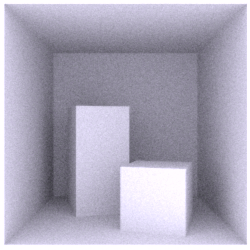
\includegraphics[width=0.2\linewidth]{Example_Scene/CornellBox_step1.png}
	\caption{Rendering result after definition of Cornell box geometry}
\end{figure}

\section{Materials and spectrums}
Now that our geometry is defined, we need to apply materials to the various elements of the scene. All the elements are considered as Lambertian in the scene. So we can use the material provided by \verb?LAMBERT_REFLECTOR_CONST?. This needs a spectrum to be constructed. For the lighting, \verb?LAMBERT_EMITTER? is going to be used.

\paragraph{Constructing spectrums} Various choices for constructing spectrums exists in ART. Since the provided spectrums in the specification are regularly sampled, we can use \verb?CONST_COLOUR_RSSPECTRUM? define which takes the starting wavelength, the sampling step, a maximum value used for normalisation and the list of values for the spectrum.

So, we have:
\begin{lstlisting}
ArObj whiteReflectance(ART_GV * art_gv) {
    return 
        CONST_COLOUR_RSSPECTRUM(400 NANOMETER, 4 NANOMETER, 1.0, 
            0.343, 0.445, 0.551, 0.624, 0.665, 0.687, 0.708, 0.723, 0.715, 
            0.710, 0.745, 0.758, 0.739, 0.767, 0.777, 0.765, 0.751, 0.745, 
            0.748, 0.729, 0.745, 0.757, 0.753, 0.750, 0.746, 0.747, 0.735, 
            0.732, 0.739, 0.734, 0.725, 0.721, 0.733, 0.725, 0.732, 0.743, 
            0.744, 0.748, 0.728, 0.716, 0.733, 0.726, 0.713, 0.740, 0.754, 
            0.764, 0.752, 0.736, 0.734, 0.741, 0.740, 0.732, 0.745, 0.755, 
            0.751, 0.744, 0.731, 0.733, 0.744, 0.731, 0.712, 0.708, 0.729, 
            0.730, 0.727, 0.707, 0.703, 0.729, 0.750, 0.760, 0.751, 0.739, 
            0.724, 0.730, 0.740, 0.737, RSS_END
            );
}

ArObj greenReflectance(ART_GV * art_gv) {
    return
        CONST_COLOUR_RSSPECTRUM(400 NANOMETER, 4 NANOMETER, 1.0, 
            0.092, 0.096, 0.098, 0.097, 0.098, 0.095, 0.095, 0.097, 0.095, 
            0.094, 0.097, 0.098, 0.096, 0.101, 0.103, 0.104, 0.107, 0.109, 
            0.112, 0.115, 0.125, 0.140, 0.160, 0.187, 0.229, 0.285, 0.343, 
            0.390, 0.435, 0.464, 0.472, 0.476, 0.481, 0.462, 0.447, 0.441, 
            0.426, 0.406, 0.373, 0.347, 0.337, 0.314, 0.285, 0.277, 0.266, 
            0.250, 0.230, 0.207, 0.186, 0.171, 0.160, 0.148, 0.141, 0.136, 
            0.130, 0.126, 0.123, 0.121, 0.122, 0.119, 0.114, 0.115, 0.117, 
            0.117, 0.118, 0.120, 0.122, 0.128, 0.132, 0.139, 0.144, 0.146, 
            0.150, 0.152, 0.157, 0.159, RSS_END
            );
}

ArObj redReflectance(ART_GV * art_gv) {
    return
        CONST_COLOUR_RSSPECTRUM(400 NANOMETER, 4 NANOMETER, 1.0, 
            0.040, 0.046, 0.048, 0.053, 0.049, 0.050, 0.053, 0.055, 0.057, 
            0.056, 0.059, 0.057, 0.061, 0.061, 0.060, 0.062, 0.062, 0.062, 
            0.061, 0.062, 0.060, 0.059, 0.057, 0.058, 0.058, 0.058, 0.056, 
            0.055, 0.056, 0.059, 0.057, 0.055, 0.059, 0.059, 0.058, 0.059, 
            0.061, 0.061, 0.063, 0.063, 0.067, 0.068, 0.072, 0.080, 0.090, 
            0.099, 0.124, 0.154, 0.192, 0.255, 0.287, 0.349, 0.402, 0.443, 
            0.487, 0.513, 0.558, 0.584, 0.620, 0.606, 0.609, 0.651, 0.612, 
            0.610, 0.650, 0.638, 0.627, 0.620, 0.630, 0.628, 0.642, 0.639, 
            0.657, 0.639, 0.635, 0.64, RSS_END
            );
}

ArObj lightSpectrum(ART_GV * art_gv) {
    return 
        CONST_COLOUR_RSSPECTRUM(400 NANOMETER, 100 NANOMETER, 1.0,
            0.0, 8.0, 15.6, 18.4,
            RSS_END
            );

}
\end{lstlisting}

\paragraph{Assigning material to objects}
Let's first assign the material to the two bocks. We are using a \verb?LAMBERT_REFLECTOR_CONST? with the spectrum provided by the function \verb?whiteReflectance? for reflectance. To assign a material to an object, we use the method \verb?apply?.

This method can take several types, or subnodes, so, we just need to add another material subnode before returning the obects:

\begin{lstlisting}
ArObj createShortBlock(ART_GV * art_gv) {
    ...
    
    id blockMaterial = LAMBERT_REFLECTOR_CONST(whiteReflectance(art_gv));

    return 
        [ block apply
            : vertices
            : blockMaterial
            ];
}

ArObj createTallBlock(ART_GV * art_gv) {
    ...
    
    id blockMaterial = LAMBERT_REFLECTOR_CONST(whiteReflectance(art_gv));
    
    return 
        [ block apply
            : vertices
            : blockMaterial
            ];
}
\end{lstlisting}

For the walls, each of them have a different reflectance. Then, the \verb?apply? method must by called on the \verb?QUADRANGLE?.

\begin{lstlisting}
ArObj createBox(ART_GV * art_gv) {
    ...

    id whiteLambert = LAMBERT_REFLECTOR_CONST(whiteReflectance(art_gv));
    id redLambert   = LAMBERT_REFLECTOR_CONST(redReflectance(art_gv));
    id greenLambert = LAMBERT_REFLECTOR_CONST(greenReflectance(art_gv));

    ArObj floorGeometry = 
        [ QUADRANGLE(2, 3, 1, 6) apply
            : whiteLambert
            ];

    ArObj ceilingGeometry =
        [ QUADRANGLE(4, 5, 1, 0) apply
            : whiteLambert
            ];

    ArObj rightWallGeometry =
        [ QUADRANGLE(6, 7, 5, 4) apply
            : greenLambert
            ];

    ArObj leftWallGeometry = 
        [ QUADRANGLE(0, 1, 3, 2) apply
            : redLambert
            ];

    ArObj backWallGeometry =
        [ QUADRANGLE(2, 0, 4, 6) apply
            : whiteLambert
            ];

    ArObj box =
        UNION(
            floorGeometry,
            rightWallGeometry,
            ceilingGeometry,
            leftWallGeometry,
            backWallGeometry,
            UNION_END
            );

    return [ box apply: vertices ];
}
\end{lstlisting}

Let's create now our lighting. The same way as we've build our geometry and assigned a material to the objects of the scene, the lighting will consist in a single \verb?QUADRANGLE? indexing some vertices. Then, we apply a \verb?LAMBERT_EMITTER? to it:

\begin{lstlisting}
ArObj ceilingHoleGeometry(ART_GV * art_gv) {
    Pnt3D * ceilingHolePoints = ALLOC_ARRAY(Pnt3D, 5);


    ceilingHolePoints[0] = PNT3D( 343.0, 548.8 , 227.0);
    ceilingHolePoints[1] = PNT3D( 343.0, 548.8 , 332.0);
    ceilingHolePoints[2] = PNT3D( 213.0, 548.8 , 332.0);
    ceilingHolePoints[3] = PNT3D( 213.0, 548.8 , 227.0);

    ceilingHolePoints[4] = PNT3D_HUGE;
    
    ArObj vertices =
        arnvertexset(
            art_gv,
            ceilingHolePoints,
            NULL,
            NULL,
            NULL,
            NULL
            );

    return [ QUADRANGLE( 0, 1, 2, 3 ) apply: vertices ];
}

ArObj createLight(ART_GV * art_gv) {
    ArObj emitterMaterial = LAMBERT_EMITTER( lightSpectrum(art_gv), 1.0 );

    return [ ceilingHoleGeometry(art_gv) apply: emitterMaterial ];
}
\end{lstlisting}

Now, we can remove the \verb?environmentMaterial? from the scene and render the file.

\lstinputlisting{Example_Scene/CornellBox.arm}

\begin{figure}[h]
	\centering
	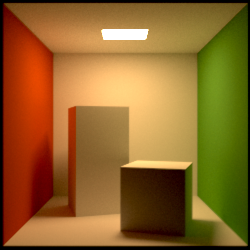
\includegraphics[width=0.2\linewidth]{Example_Scene/CornellBox.png}
	\caption{Rendering result of the Cornell box scene}
\end{figure}

\section{Defines}
You may notice that the previous scene contains a define for specifying the number of samples. You can use define the same way you would use it with a standard compiler. This enables you to bring flexibility to your scene.

So, in our example, to specify to the renderer to use 128 samples, you simple invoke \verb?artist? this way:

\begin{verbatim}
artist CornellBox.arm -DSAMPLES=128
\end{verbatim}


\part{ARM Defines and Functions}
\subimport{generated/}{ARM_Interface_gen.tex}

\end{document}
